\chapter{Supplementary materials for \autoref{chap:CMZ}}
\section{Description of the computational cluster used in the work}
\label{cluster}

\section{Developmental progression of naso-temporal population asymmetry in the CMZ}

\begin{figure}[!h]
    \makebox[\textwidth][c]{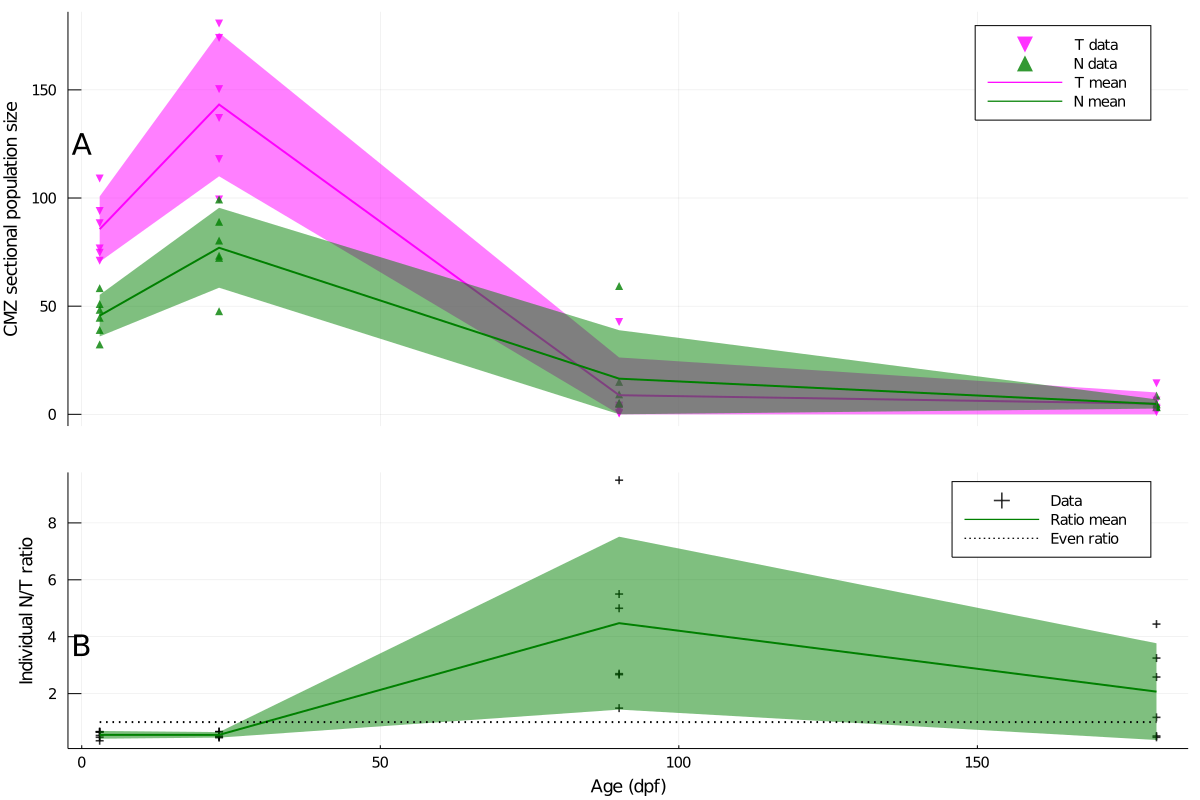
\includegraphics[width=1.2\textwidth]{cmz/NTontology.png}}    
    \caption{{\bf Developmental progression of naso-temporal population asymmetry in the CMZ.}}
    Marginal posterior distribution of mean nasal (N) and temporal (T) population size in 14$\mu$m transverse cryosections (panel A) or intra-individual N/T count asymmetry ratio (panel B), $\pm 95\%$ credible interval, n=6 animals per age. Data points represent mean counts from three central sections of an experimental animal's eye. 
    \label{NTontology}
\end{figure}


\section{Cumulative EdU Bayesian Linear Regression}


\begin{figure}[!h]
    \makebox[\textwidth][c]{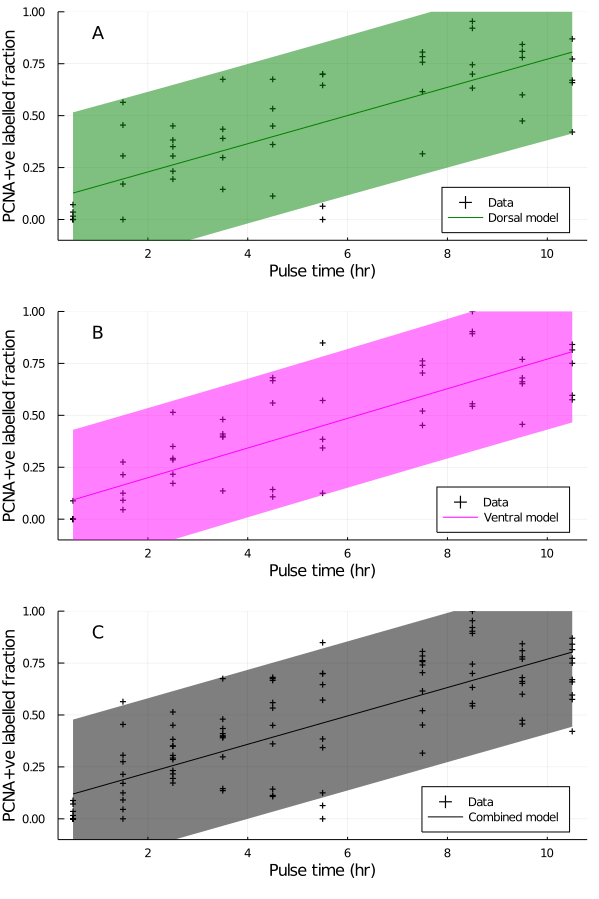
\includegraphics[width=1.2\textwidth]{cmz/3ddvlinreg.png}}    
    \caption{{\bf Linear regressions performed on cumulative labelling data from dorsal, ventral, and combined CMZ sectional populations}}
    \label{cumEdUlinreg}
\end{figure}

\section{Methods}
\label{ssec:CMZmethods}

\subsection{Statistical Analyses}


